\section{Technical Progress} 
\label{sec:technical_progress}

Continuing from the progress in the second milestone, we started implementation of the chosen visualization design. This involved a number of steps that were carried out over the course of two weeks that resulted in a visualization that now forms the basis of our future progress. The contributions made in service of this visualization design are explained in separate subsections below,

\subsection{Data Collection}
\label{sec:data collection}

The data used for the visualization was collected from the database of \textbf{Bike Share Metro}, a bike share service based in Los Angeles. This is a completely open source data that provides us with various information about any single bike ride. A more detailed description of all the fields in the data can be found in the Task Abstraction subsection of the Refinements section.\\
The data is divided into several segment, each one contained the information for a single quarter of a calendar year i.e. Q1, Q2, Q3 or Q4. After downloading the data from their online database, the resulting .zip archive was extracted. The raw data was provided in a CSV (Comma Separated Value) format.

\subsection{Data Refinement and Restructuring}
\label{sec:data refinement and restructuring}

The raw data in the CSV format is not suitable for processing and analysis. We used a more standard approach to work with data and for this the CSV data files were converted into JSON (JavaScript Object Notation) format. All of the data cleaning and pre-processing was done using the \textbf{Python} programming language. This reformatting of the raw data structure was followed by a series of further transformation which are explained in the sub-sections below.

\subsubsection{JSON Format}
As mentioned above, the first step was to convert the raw data from CSV to JSON format. Other than the structure of the data, the contents were left intact and no further manipulations were done to the data.\\
The script \texttt{csv\_to\_json.py} in the \textbf{Project} folder performs this initial conversion.

\subsubsection{GeoJSON Format}
While the JSON data format in itself is pretty suitable for data analysis and works very well for our purposes, GeoJSON is a format that works even better when visualizations involve geographic maps and latitude, longitude locations. During this process, we also performed data cleaning operations where data containing incomplete information were not loaded into the GeoJSON data structure.\\
The script \texttt{json\_to\_geojson.py} in the \textbf{Project} folder converts the JSON file into a GeoJSON data structure.

\subsubsection{Task-Specific Formats}
Following the GeoJSON re-formatting and data cleanup, the data structures for specific visualization mappings are created. The GeoJSON file is taken as the base file from which all other dictionaries and arrays of information are extracted.\\
For our current visualization progress, we have a single extraction from the GeoJSON file. This dictionary contains the distinct geographic locations of all bike pickup points along with the number of pickups for that time frame (1st quarter of 2018 in our case). This is done by the \texttt{geo\_to\_startcount.py} script in the \textbf{Project} directory.\newline\\ It should be noted that for every new visualization design or task, a new data structure will be extracted from the GeoJSON file to ease the data analysis and extraction process.
Currently, all these scripts exists in standalone and need to be executed one after the other. On the final implementation, these scripts will be a part of a single executable script which will perform all the data cleaning and manipulation tasks in a single execution.

\subsection{Data Visualization}
Following the data collection and restructuring, we proceeded towards the actual visualization of the data. The visualization process along with the different tools and packages used in support of that have been explained in the subsections below.

\subsubsection{Initial Map Layout}
The first task at hand was to lay out a map of Los Angeles over which we had to plot our data points. Though D3 in itself supports drawing maps, we required a detailed street level map layout. For this purpose, D3 could not be used alone. We had to use a separate package or library that supports interactive map drawing. We had two possible options to work with for our visualization, \textbf{Google Maps API} and \textbf{Leaflet}.\\
There did not seem to be a large difference between the functionalities provided by Google Maps and Leaflet, at least for our visualization purposes. While Google Maps did was a fan favorite among a large number of developers and it did provide many added features in terms of traffic, transit data and geolocation, we decided to implement Leaflet into our project. Our decision was based on the availability and simplicity of the documentation and tutorials for these features. Leaflet conformed to our requirements smoothly and its implementation was pretty straight forward.\\
In essence, Leaflet is a open-source JavaScript library for interactive maps \cite{Leaflet:2017:Doc}. It is light weight and consists of a plethora of features that can be implemented for interactive map visualizations. For our visualization, we create the map in the 'map' div and add \textit{OpenStreetMap} tiles to load the map area. As a starting point, we provide the map with a fixed co-ordinate and a zoom level. Using this information, an initial visual representation of the map is obtained. From here, users can further interact with the map. The interactions supported in our visualization are discussed in detail in a later section.
\begin{figure}[h]
	\centering % avoid the use of \begin{center}...\end{center} and use \centering instead (more compact)
	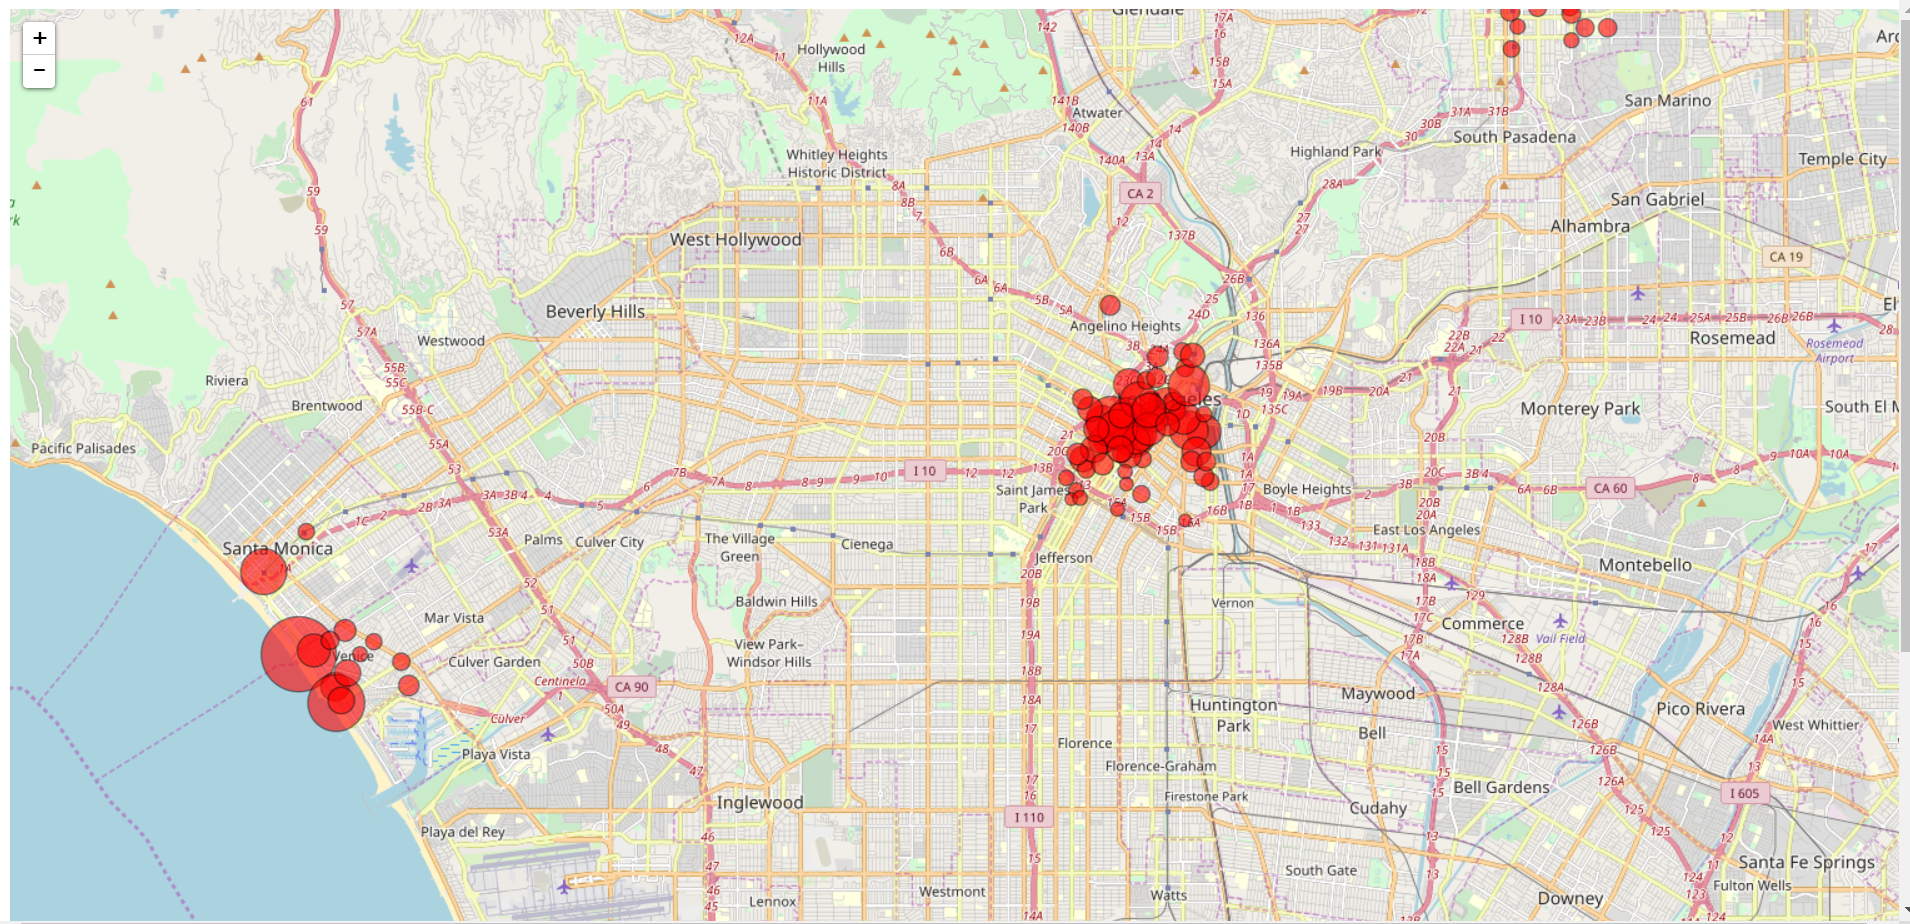
\includegraphics[scale=0.20]{figs/highlevel.PNG}
	\caption{\footnotesize{A high-level overview of current visualization}}
	\label{fig:First viz Chart}
	\captionsetup{justification=centering,margin=1cm}
	\vspace{-10pt}
\end{figure}
\subsubsection{Data Plotting}
After plotting the map of Los Angeles, we started with plotting the data points over this map. For the first visualization, we plotted the starting locations of all bike rides over the map. These were distinct locations in the map, defined by a latitude and longitude value. We used the data for the 1st quarter of 2018 as our seed data. The number of data points were in the order of 60,000 for a single quarter. For now, this data is loaded locally but as we include more data points for different quarters and years, we are planning to shift the data loading through a web server. This will considerably decrease the load time of the visualization.\\
The data points for our visualization are represented as circles of varying area (radius). The data is encoded in such a way that the radius linearly increases with the frequency of bike pick-ups for a given location. We keep the opacity of the circles to a value less than 1 so as to make the map visualization easier to understand and navigate. These circles are stroked with a minimum thickness to make them stand out when viewing from a zoomed-out perspective.
\begin{figure}[h]
	\centering % avoid the use of \begin{center}...\end{center} and use \centering instead (more compact)
	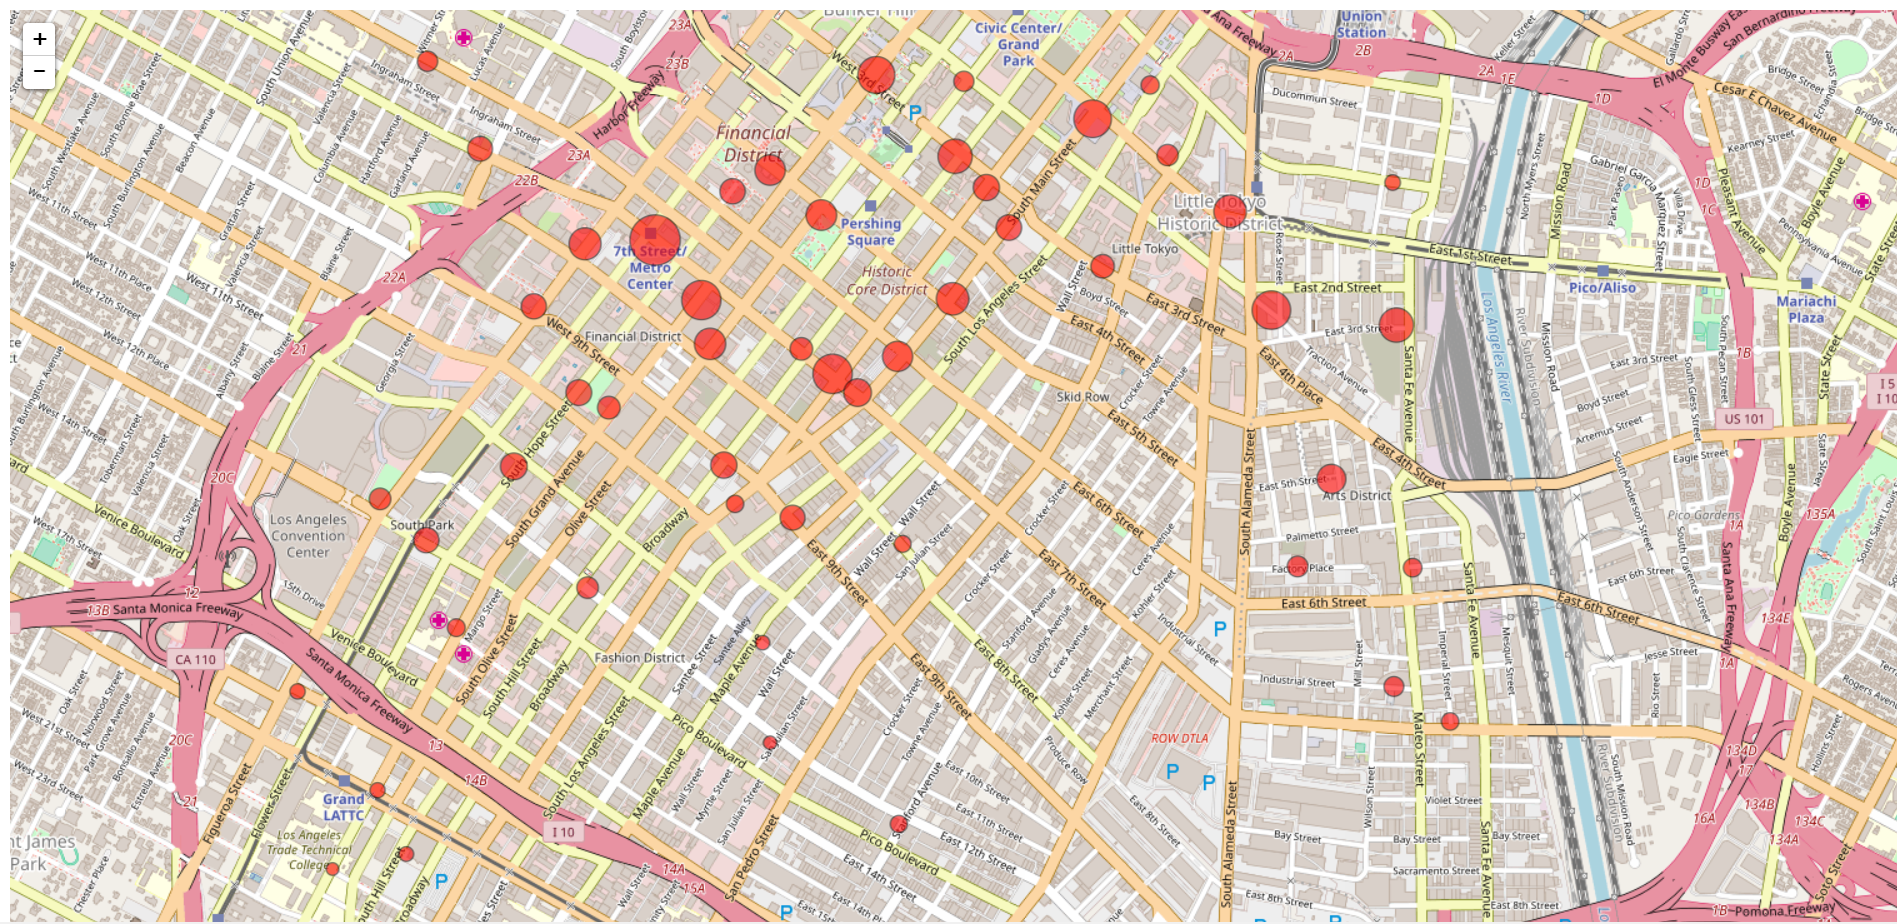
\includegraphics[scale=0.20]{figs/zoomedin.PNG}
	\caption{\footnotesize{A zoomed in view showing distinct geographic points}}
	\label{fig:First viz Chart}
	\captionsetup{justification=centering,margin=1cm}
	\vspace{-10pt}
\end{figure}
\subsection{User Interaction}
Our visualization design currently supports a number of interactions. These visualizations have been presented in the short movie as well. As work progresses on the visualization, these interactions will be enhanced and others added. For now, the following interactions are available to the user:
\begin{itemize}
    \item \textbf{Panning and Zooming}: The geographic map can be panned sideways to move around and locate different data points around the city. Also, the map can be zoomed in and out. Zooming in allows users to get a closer look into the data points on a street level view. This way the bike stations look more distinguishable from one another. The zoom feature here is constrained and semantic in nature. This interaction follows the Shneiderman's mantra of having an overview first and then allowing to zoom in and filter data.
    \item \textbf{Pop-up Effect}: The individual data points support a "On Click" feature. Every time a data point i.e. a circle is clicked, the color of the circle changes to blue with a more defined stroke around the circle. This makes the data point more visible and allows it to stand out, especially when there are a large number of similar data points around it. We decided on choosing the "On Click" action to show the effect rather than the "Hover" action since clicking an element to have a detailed overview of a single data point is more effective than hovering over it. Either ways, this follows the Shneiderman's Detail-on-Demand task taxonomy.
    \item \textbf{Tooltip}: In addition to the "On Click" feature changing the color of the circle, a tooltip will also appear on top of each data point. Currently, this tooltip shows the number of bike pick ups for a given location but a future enhancement might be to add a small visualization pertaining to the data within that geographic point.
\end{itemize}
\begin{figure}[h]
	\centering % avoid the use of \begin{center}...\end{center} and use \centering instead (more compact)
	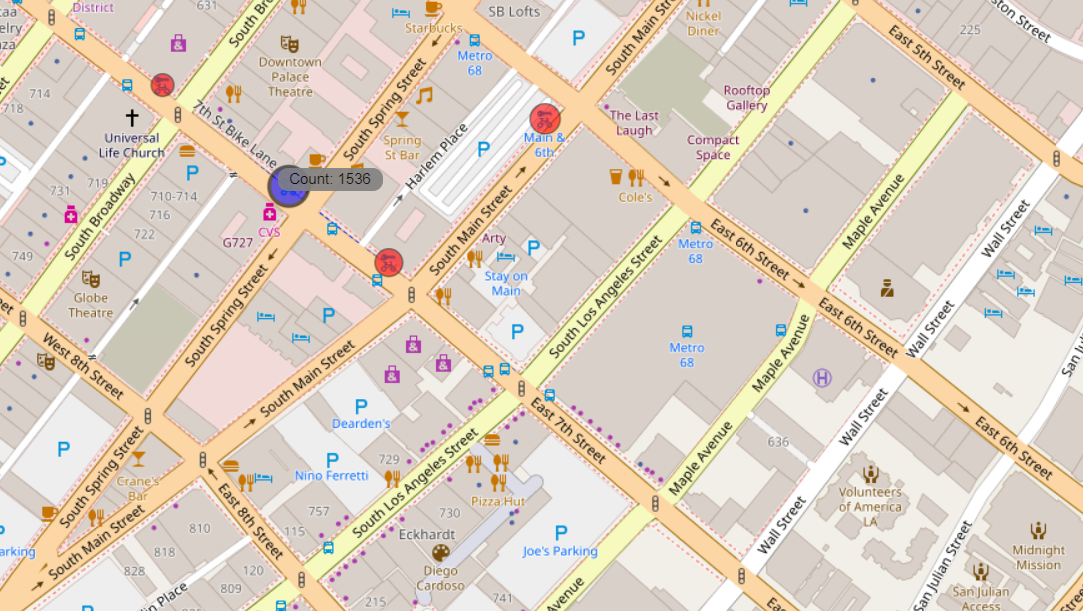
\includegraphics[scale=0.36]{figs/tooltip.png}
	\caption{\footnotesize{A simple tooltip implementation}}
	\label{fig:First viz Chart}
	\captionsetup{justification=centering,margin=1cm}
	\vspace{-10pt}
\end{figure}
This visualization has been coded by dividing the structure of the program into 3 segments:
\begin{itemize}
    \item PM3.html
    \item PM3.js
    \item PM3.css
\end{itemize}
As work progresses on the visualization, we plan on adding a histogram time frame at the bottom of the visualization window. This histogram will stretch the width of the window and allow users to cross-filter data in the map based on the selection in the histogram window.